% Please use the skeleton file you have received in the
% invitation-to-submit email, where your data are already
% filled in. Otherwise please make sure you insert your
% data according to the instructions in PoSauthmanual.pdf
\documentclass{PoS}

\title{Studies of the microwave emission of extensive air showers with EASIER and MIDAS at the Pierre Auger Observatory}

\ShortTitle{MBR emission at Auger}

\author{\speaker{Romain Gaior}$^a$ for the Pierre Auger Collaboration$^b$\\
\llap{$^a$}Your Institution Affiliation, City, Country\\
\llap{$^b$}Observatorio Pierre Auger, Av.\ San Mart\'in Norte 304, 5613 Malarg\"ue, Argentina\\
E-mail: \href{mailto:auger_spokespersons@fnal.gov}{\rm auger\_spokespersons@fnal.gov}\\
Full author list: \href{http://www.auger.org/archive/authors_icrc_2017.html}{\rm http://www.auger.org/archive/authors\_icrc\_2017.html}}

\abstract{Your full abstract comes here.}

\FullConference{35th International Cosmic Ray Conference\\
                10--20 July, 2017\\
                Bexco, Busan, Korea}



\begin{document}

\section{Introduction}
The measurement of the composition of the Ultra High Energy Cosmic Rays (UHECR) is crucial to constrain their origin. The two main techniques to characterize the Extensive Air Shower (EAS) induced by the UHECR, is either a particle detector array at ground or a fluorescence telescope. Unfortunately, in their actual form, the particle detector at ground are limited in their sensitivity on the mass composition measurement and the fluorescence technique is sensitive to it only with a limited duty cycle of 15\% thus limiting the statistics at the highest energies. The development of 
an additional particle detector complementing the existing one is the focus of the upgrade effort undertaken at the Pierre Auger Observatory\cite{augerupgrade}.\\However, new detection channels have also been considered. The observation of the EAS through the radio waves emitted along its development in the atmosphere is one of them. Radio technique have been investigated since the 1960's and is now an experienced technique in the VHF band, a region of frequency where a strong signal is emitted in the forward direction within a Cherenkov cone of around 1 degree opening in air. This technique is now implemented in several observatories including the Pierre Auger Observatory. However the lateral extension of the radio signal doesn't allow one to instrument large area required to compensate for the very low flux at the highest energies.\\ A promising technique was proposed in 2008~\cite{gorham} after the observation of a signal in the microwave frequencies upon the passage of a particle shower in an anechoic chamber. This signal interpreted as originated from the acceleration of ionisation electrons in the molecular field, the molecular Bremsstrahlung radiation (MBR), has triggered a lot of interest. The MBR is emitted isotropically and it would allow one to measure the longitudinal profile of the EAS, as with the fluorescence but with a 100\% duty cycle. Since the first beam test results, many efforts have been undertaken, new beam test have been carried out~\cite{amy, maybe} but were not able to reproduce the initial results. Estimation of the expected signal have been improved and yielded less optimistic results. Finally, in situ experiments have tried to observe the MBR emission using existing CR observatory to probe this signal\cite{crome, icrc2013}. If clear signal were observed, their origin can be attributed to a coherent emission. In the present contribution we present the development and the results of two radio experiments, EASIER and MIDAS, installed within the Pierre Auger Observatory and able to probe the MBR emission from the UHECR.

\section{The Pierre Auger Observatory}
The Pierre Auger Observatory is an hybrid detector comprising an array of 1600 particle detectors at ground, the surface detector (SD), and a fluorescence detector (FD) measuring the fluorescence light from 5 sites surrounding the SD. Each SD station is a water cherenkov detector  equipped with a local DAQ and communication. 
The two radio detectors we present here use the same technique but are implemented in a different way. EASIER is embedded in a local SD station and intends to measure the radio waves from the ground, whereas MIDAS is inspired of the FD, and tries to measure the radiation of EAS from the side.
\begin{figure}[t]
\centering
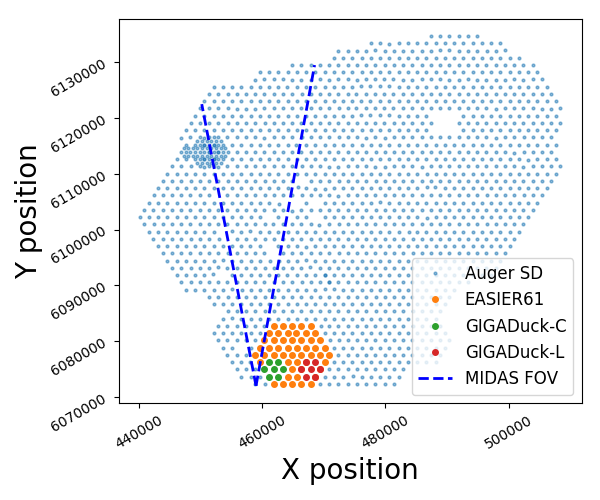
\includegraphics[width=0.4\textwidth]{layoutGHz.png}

\caption{The EASIER arrays and MIDAS field of view overlaid with the surface detector of the Pierre Auger Observatory.}
\label{fig:ghzlayout}
\end{figure}

\section{EASIER}
\subsection{Detectors}
\paragraph{Concept}
EASIER (Extensive Air Shower Identification with Electron Radiometer) is designed to observe the radio emission from EAS with an antenna looking up, and located at ground. It is operated in slave mode with an Auger SD local station and thus takes advantage of the trigger of the particle detector. The detector is composed of an antenna followed by an amplification stage and a filtering stage. The radio frequency (RF) signal is then transformed into its power envelope with a logarithmic amplifier. The output of the log amp is in turn scaled to fit into Auger SD front end where the EASIER signal replaces a low gain channel of one of the three PMTs. 
The scheme of EASIER detector is shown in the figure~\ref{fig:easierconcept}. This concept has been implemented is three different versions, two in the C-band EASIER61 and GIGADuck-C and one the L band, GIGADuck-L.
\begin{figure}[h]
\centering
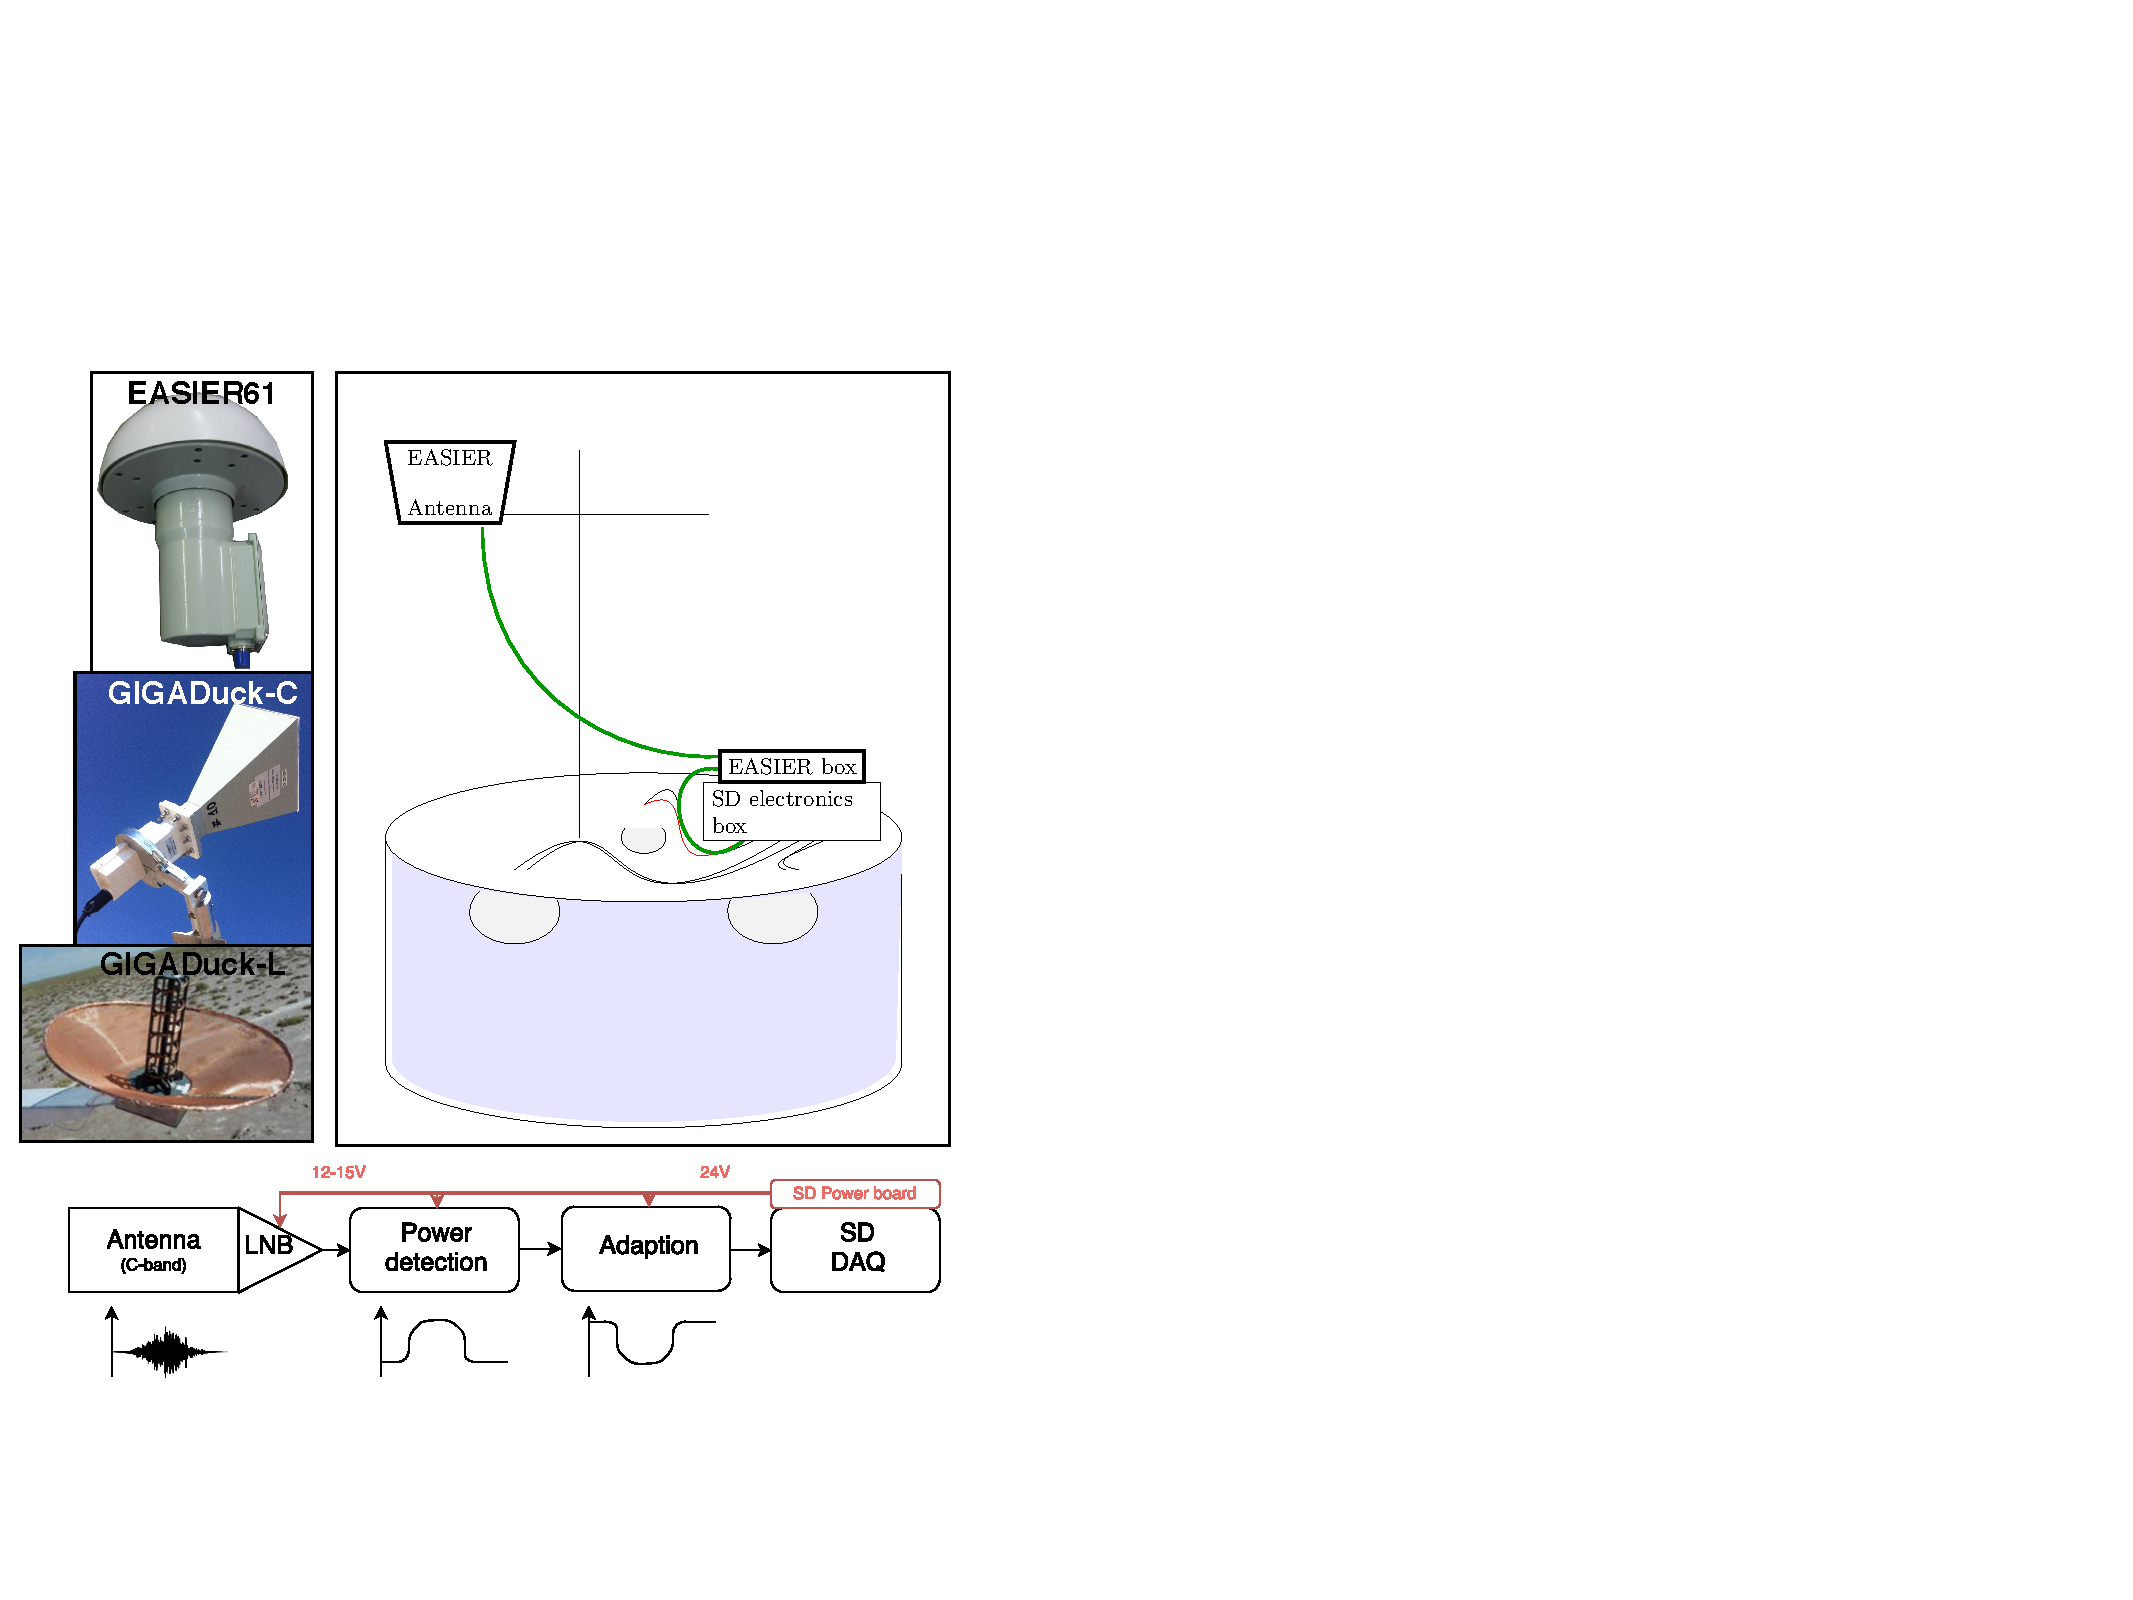
\includegraphics[width=0.4\textwidth]{easierscheme.pdf}
\caption{Scheme of EASIER concept. The sensor  placed on the tank is one the three antenna shown in the left side. The signal chain common for all the setup is represented on the bottom part.}
\label{fig:easierscheme}
\end{figure}

\paragraph{EASIER61}
The EASIER61 is the first array. A test bed of 7 antenna was installed in april 2011 and the completion to 61 detectors took place a year later. Each detector is composed of a C-band cylindrical horn antenna with a half power beam width (HPBW) of 90$^\circ$. The antenna point toward the zenith. EASIER61 has measured clear events in coincidence with the particle detector. However, because of the geometry configuration of these events, a short distance to the shower axis, or  inclined events, the origin of this signal can be attributed to coherent processes.
\paragraph{GIGADuck-C}
GIGADuck is an improvement of the EASIER detector. It is an array of seven detectors instrumented with a larger gain antenna, to increase the sensitivity to MBR, and an optimized geometry to enhance the coincidence probability between radio detectors. This design was implemented in the C-band and the L-band. In the C-band, the antenna is a pyramidal horn with 15dB gain and a HPBW of 60$^\circ$, followed by an LNB (Norsat 8115F). Each antenna points in a different direction, the central one looks at the zenith while the other six are tilted by 20$^\circ$ and have their azimuth to be oriented in the direction of the central detector. A coincidence between two detectors would favour the MBR origin of a signal against a coherent process.
\paragraph{GIGADuck-L}
The GIGADuck design has been implemented in the L-band as well. The antenna is now a helix antenna with a maximum gain at 1.4GHz and a HPBW of 60$^\circ$. Contrary to the two other setup, we developed the amplification board. A low noise amplifier board was designed with a Electric Surge protection at the input, a band pass filter, and two amplifier in chain. 
\begin{figure}[h]
\centering
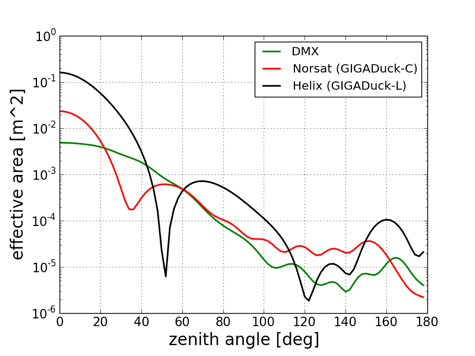
\includegraphics[width=0.4\textwidth]{effectiveareas.png}
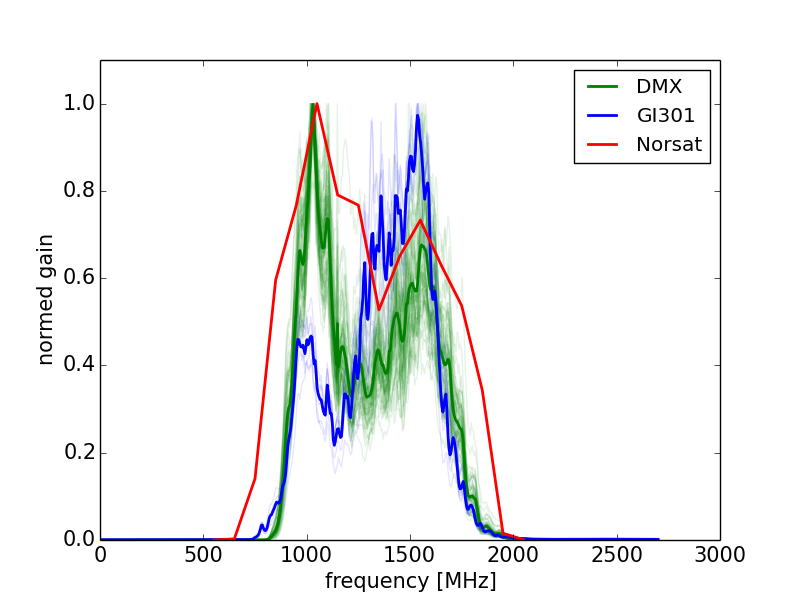
\includegraphics[width=0.4\textwidth]{spectra3.png}

\caption{Scheme of EASIER concept. The sensor  placed on the tank is one the three antenna shown in the left side. The signal chain common for all the setup is represented on the bottom part.}
\label{fig:calib}
\end{figure}
\subsection{Detector calibration}
The sensitivity of a radio power detector like EASIER can be estimated with the figure of merit that defines approximately the minimum flux one can detect:
\begin{equation}
	\rm	F_{min} = \frac{k_{B}T_{sys}}{A_{eff}\sqrt{\Delta \nu \Delta t}}
\end{equation}
where the $\rm T_{sys}$ is the system temperature, $\rm A_{eff}$ the effective area, $\rm Delta \nu$ and $\rm Delta t$ the bandwidth and the time over which the signal can be integrated.\\
The measured bandwidths and the simulated effective area of the three C-band detectors are shown in the figure~\ref{fig:calib}. One can see that the lobes of the GIGADuck detectors are more focused. \\ The system temperature is more difficult to measure. For the three setups it was actually measured with a different method. For EASIER61 detectors it was estimated with a simple dedicated measurement, we simply measured detector output when pointed to the sky and when oriented towards the ground. From the power difference between these two measurements, the intrinsic system temperature can be measured (the so called Y-factor method). For the GIGADuck-C band, we have developped a method using the sun as a calibration source. A radio baseline from the monitoring data is shown in the figure~\ref{fig:monit} top together with the ambiant temperature in blue. One can clearly see on the bottom plot  of the same figure, once the temperature dependence was removed, the bump whose origin is the solar flux. This bump can be fitted with a second order polynomials and a gaussian function. For three of the seven antennas installed we have selected a set of days when the sun is in their field of view and measured the sun contribution. The expected contribution of the sun  is computed combining the measured solar flux from the Nobeyama Observatory~\cite{bib:nobeyama} and the simulated effective area of the antenna. Hence we have:
\begin{equation}
	\rm	\frac{P_{on}}{P_{off}} = \frac{k_{B}T_{sys} + F_{sun}A_{eff}}{k_{B}T_{sys}}
\end{equation}
The baseline of the helix detectors exhibit also a clear bump attributed to the sun. However other contributions can be noticed along the day (see figure~\ref{fig: baseline}). These modulations are likely to be signal from positioning satellite which all emit in the L-band and prevent us to isolate the sun signal. We thus estimate the system temperature directly from the calibration made prior the installation.
\begin{center}
  \begin{tabular}{ | c | c | c | c | c |}
    \hline
	& antenna & geometry & fov / Aeff max & system temperature \\ \hline
	EASIER61 & C-band cylindrical horn & (0,0) & 90 / $10^-3$ & 100 K\\ \hline
	GIGADuck-C & C-band pyramidal horn & 6 tilted 1 vertical  & 60 / $10^-2$ & 50 K\\ \hline
	GIGADuck-L & L-band helix & 6 tilted 1 vertical  & 60 / $10^-1$ & 100 K\\ \hline
  \end{tabular}
\end{center}
\begin{figure}[h]
\centering
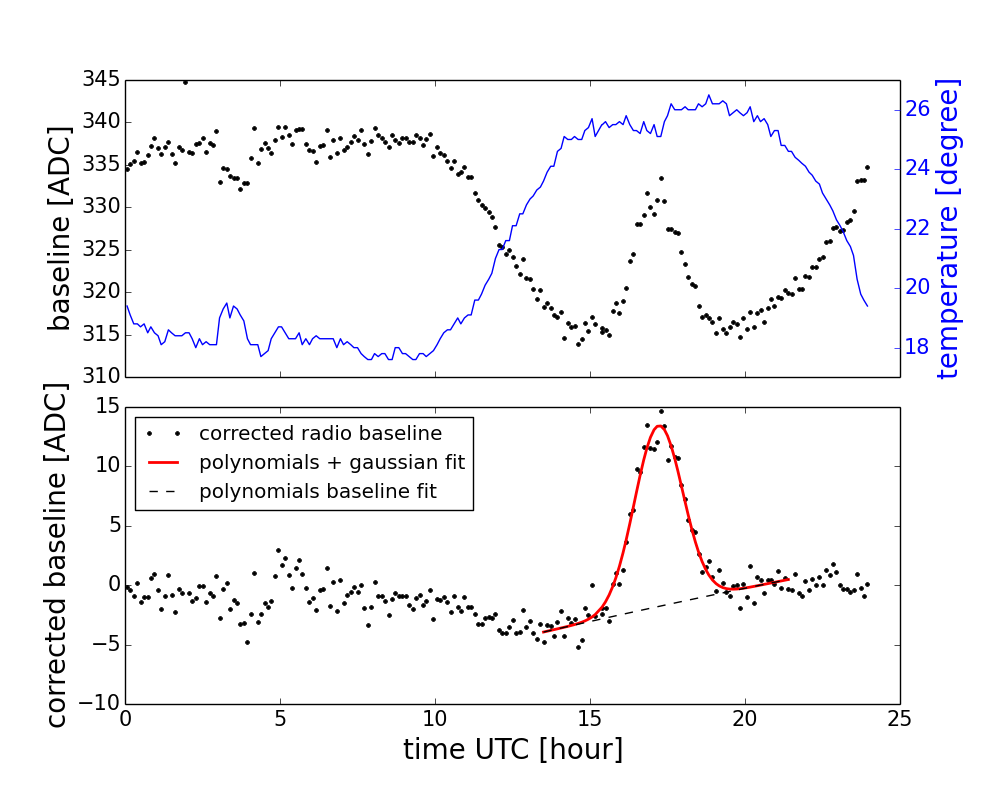
\includegraphics[width=0.4\textwidth]{newfitexamp.png}
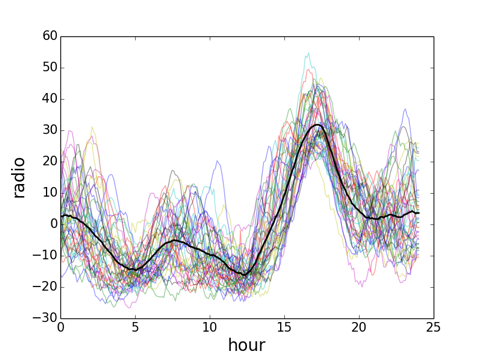
\includegraphics[width=0.4\textwidth]{jorgehour.png}

\caption{Scheme of EASIER concept. The sensor  placed on the tank is one the three antenna shown in the left side. The signal chain common for all the setup is represented on the bottom part.}
\label{fig:baselines}
\end{figure}
\subsection{Results}
The EASIER arrays have recorded data together with the Auger normal stream from 6 years for the EASIER61 array to 6 month for GIGADuck-L array, the last installed. We show in this section a search for radio event in coincidence with EAS recorded by the Auger SD.\\We build a data set from the Auger data, and we proceed to a first selection on the cosmic ray event quality i.e. regular cuts on the reconstruction and the removal of events tagged as lightning. A second set of cuts is applied on the radio trace caracteristics, we remove traces with large RMS or with more than 10 bins saturated (out of 768). 

\paragraph{Event search}
The data set is split in a $background set$ composed of the station with a distance larger than 3km from the shower axis and a $signal set$ which select among the EAS event of energy larger than 5 EeV and zenith angle smaller than 60$^{\circ}$ the station closer than 2km from the shower axis. The distribution of the radio maximum as a function of the time of this maximum is shown in the figure~\ref{fig:searchres} for the 4 setups. One can see a clear accumulation of event with large radio signal at the time bin 240 which is only 100ns before the SD trigger. To extract the radio events, we determine a threshold from the background sample which impose 99.7\% of the events to have a lower radio maximum than this threshold. A time condition is also set so that the time of maximum is inside 500ns around the particle trigger.
\begin{figure}[h]
\centering
%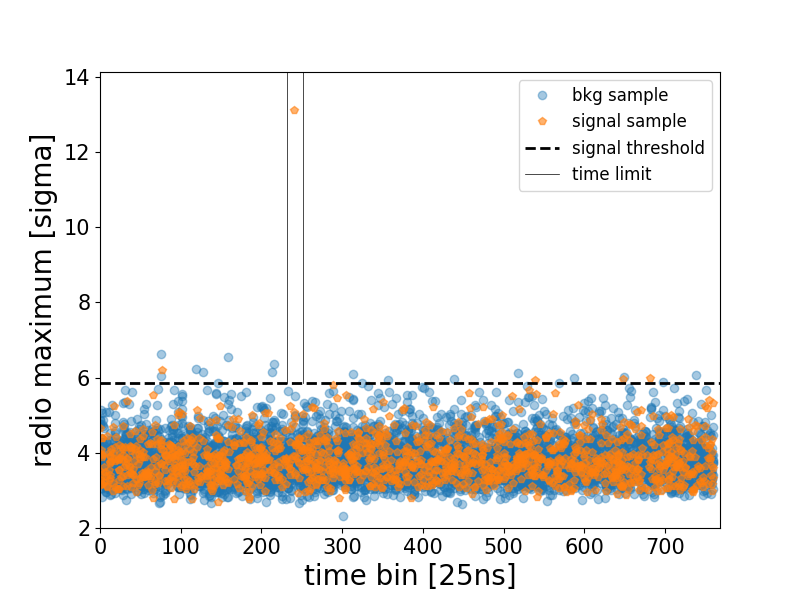
\includegraphics[width=0.24\textwidth]{EA7_event.png}
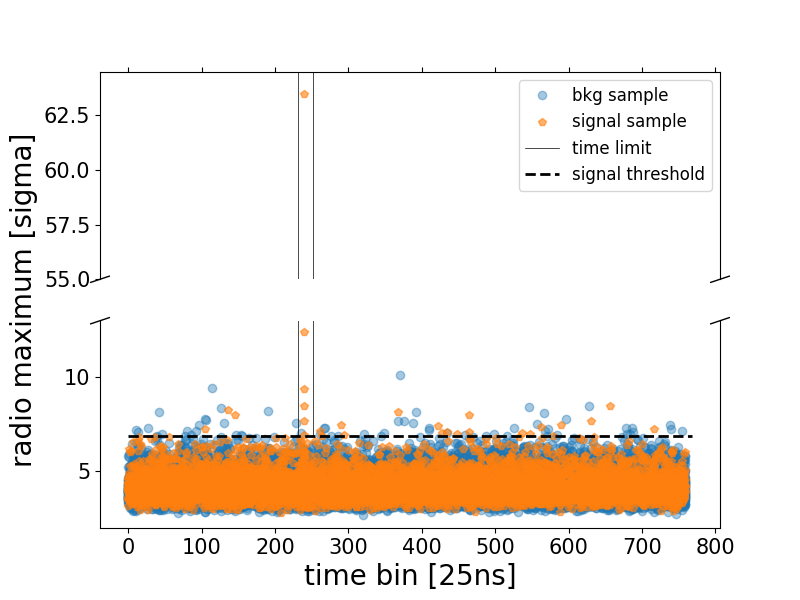
\includegraphics[width=0.32\textwidth]{EA61_event.png}
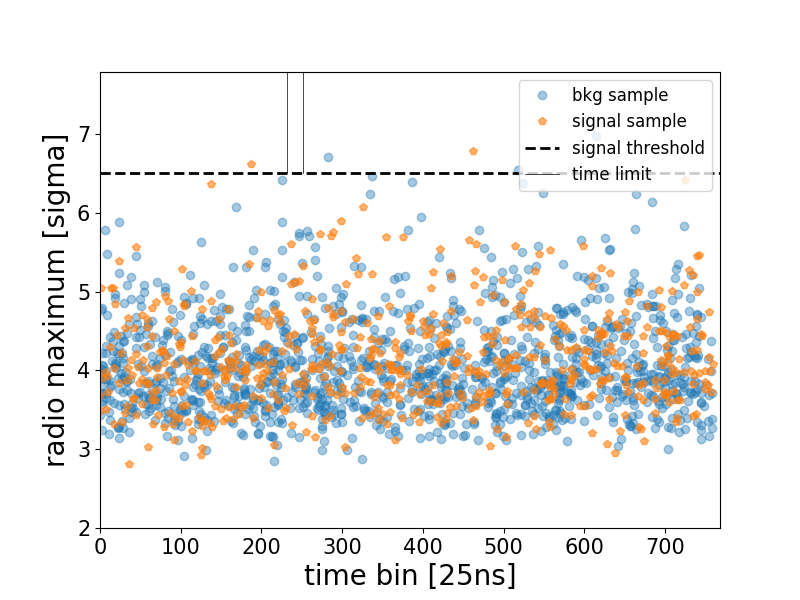
\includegraphics[width=0.32\textwidth]{GDC_event.png}
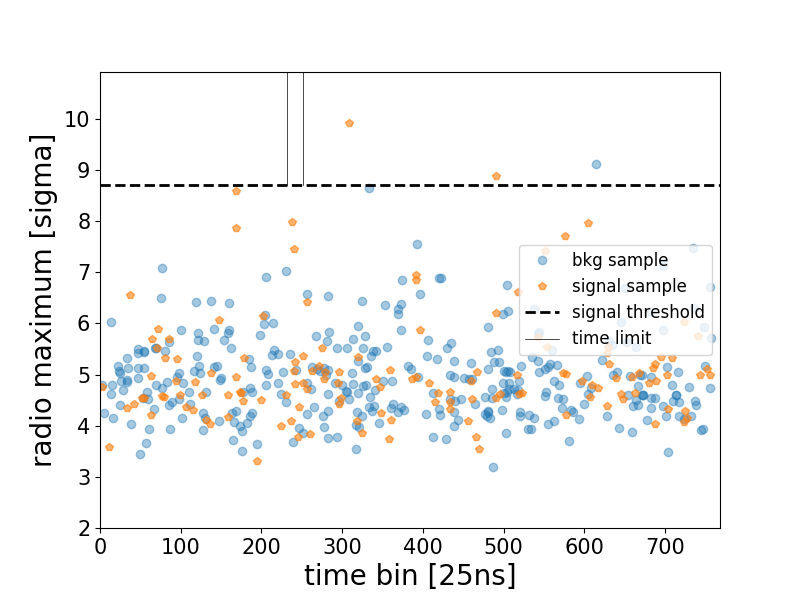
\includegraphics[width=0.32\textwidth]{GDL_event.png}
\caption{Scheme of EASIER concept. The sensor  placed on the tank is one the three antenna shown in the left side. The signal chain common for all the setup is represented on the bottom part.}
\label{fig:eventsearch}
\end{figure}
Events are found only in the EASIER61 setup where event with radio signal up to 63 sigma are recorded. The parameters of these events are listed in the Table~\ref{tab:eventlist}. A striking caracteristic is the short distance of all the detected events. 

\paragraph{Event characteristics}
\paragraph{Discussion}


\section{MIDAS}
\begin{figure}[h]
\centering
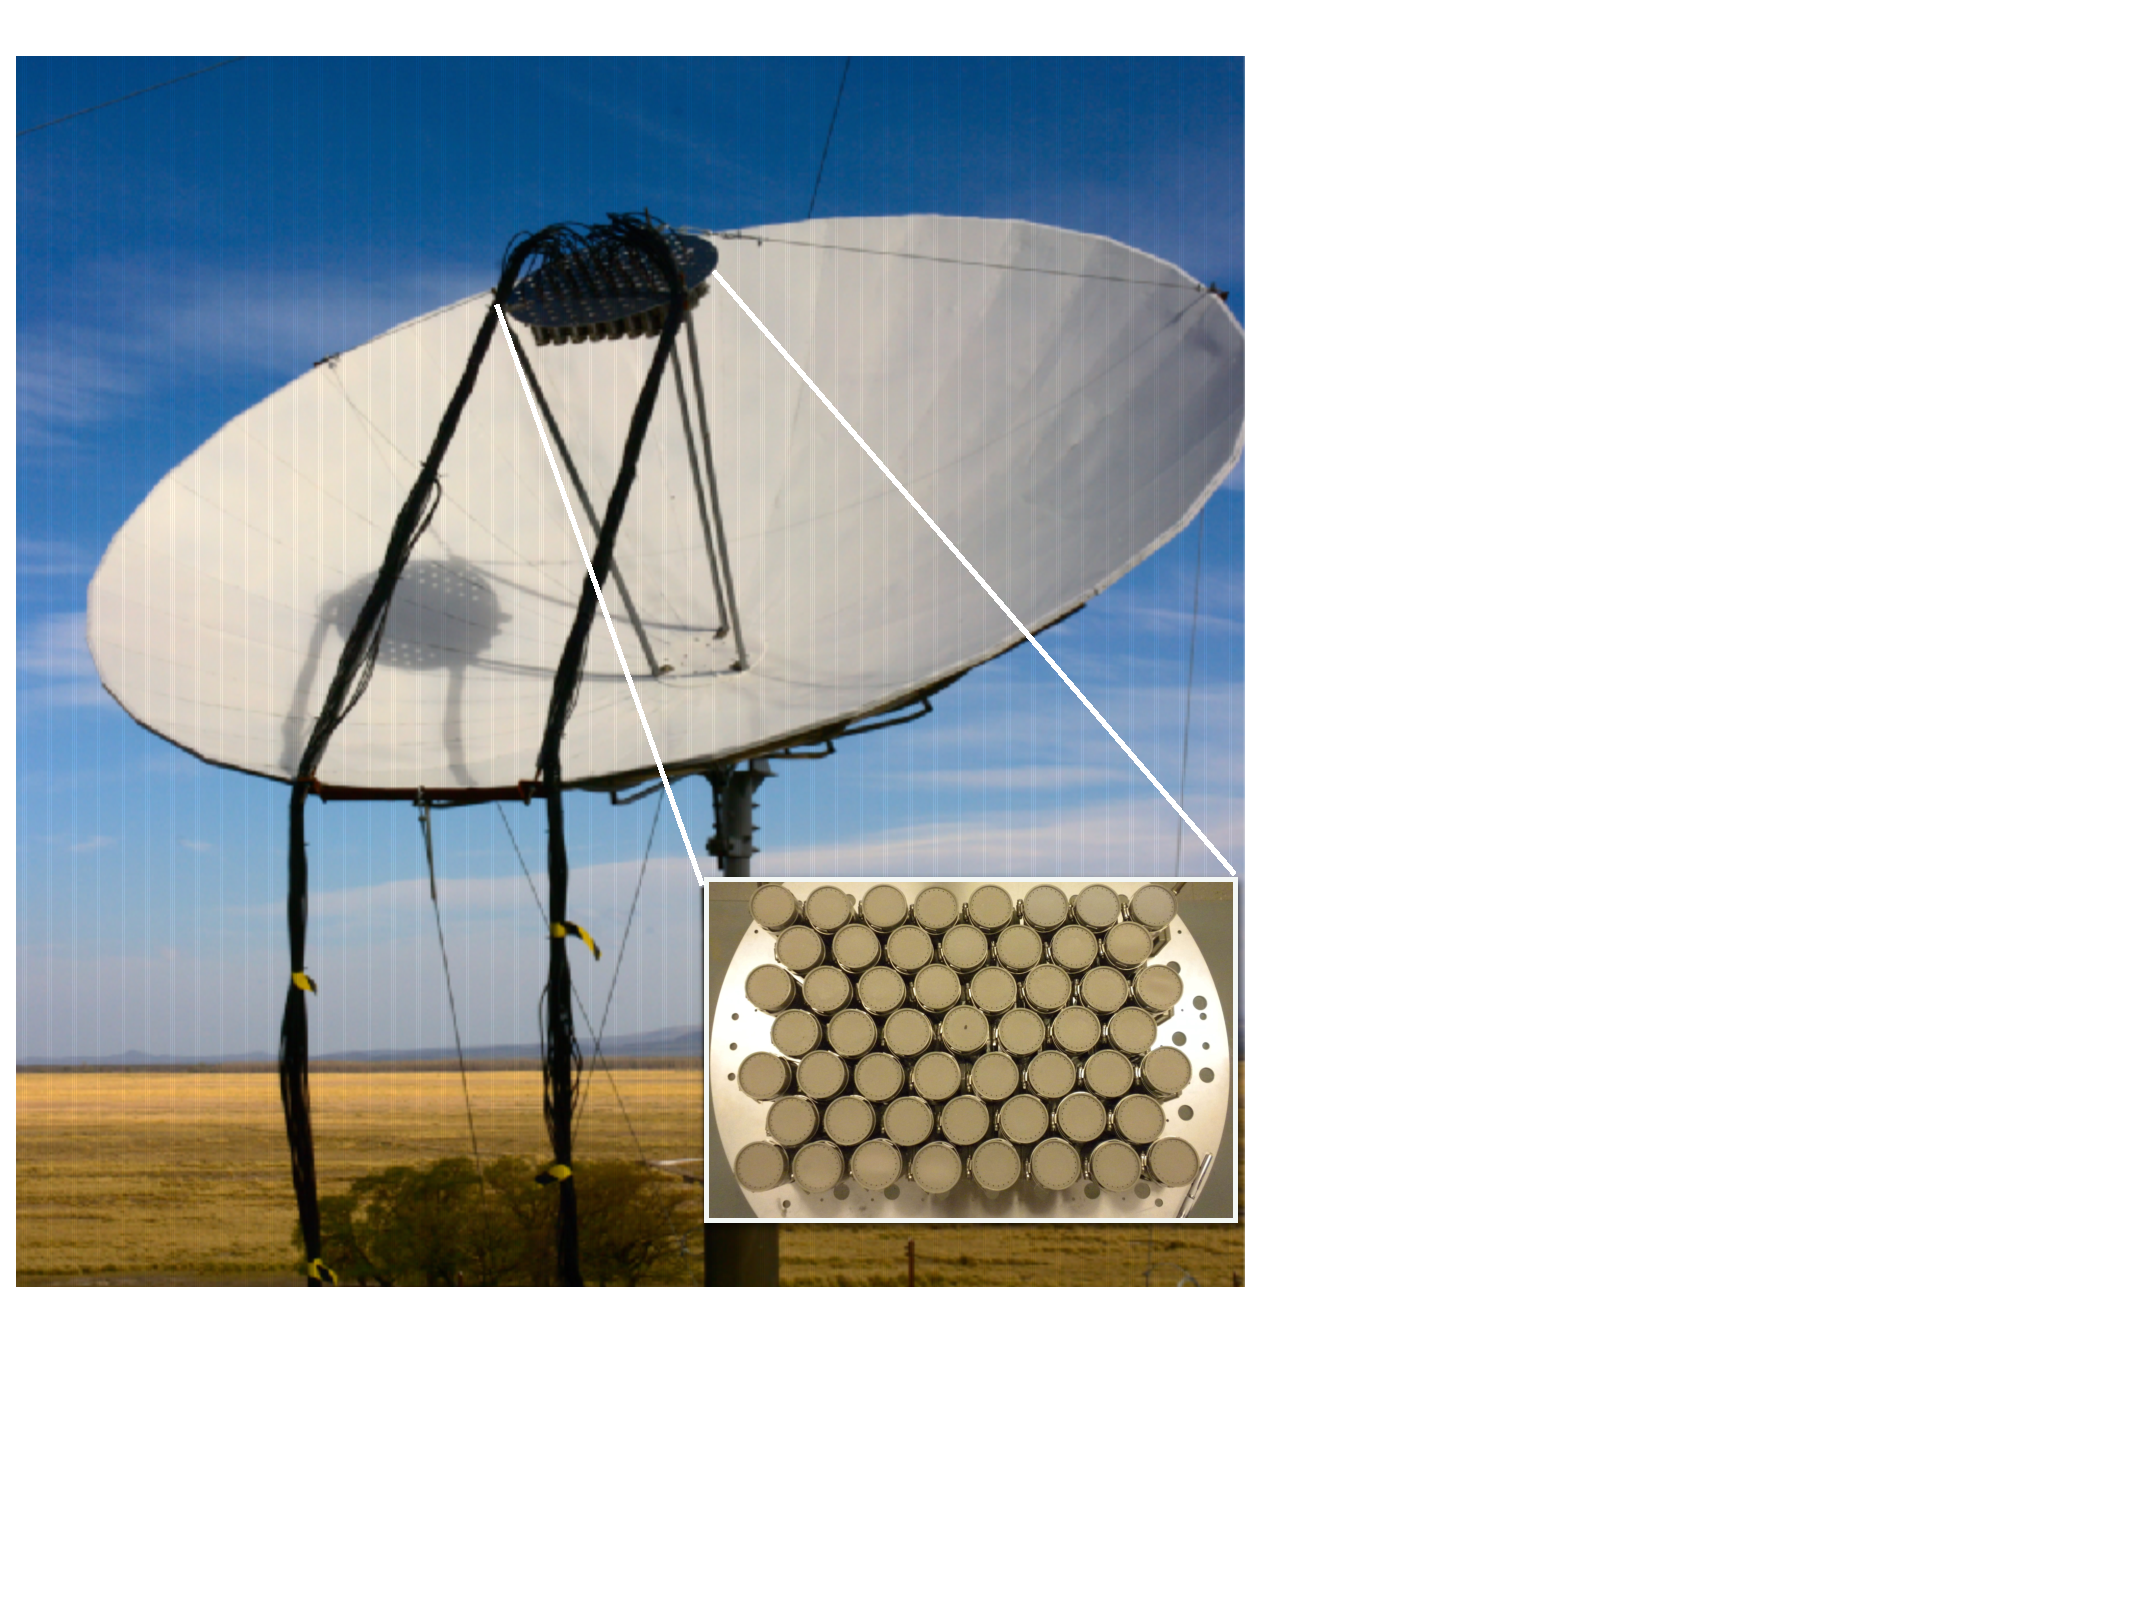
\includegraphics[width=0.6\textwidth]{midasdet.pdf}

\caption{Scheme of EASIER concept. The sensor  placed on the tank is one the three antenna shown in the left side. The signal chain common for all the setup is represented on the bottom part.}
\label{fig:baselines}
\end{figure}
\subsection{Detectors}
The MIDAS detector, first commissioned at the University of Chicago in 2010~\cite{bib:midaschicago} and currently installed at the Pierre Auger Observatory as seen in ??.  Equipped with a 5 m diameter parabolic antenna with a 53 pixel camera at its focus (3.2), the design of the MIDAS telescope is analogous to the design of one of the FDs at the Auger observatory as explained in § 1.3.1. Collectively, the 53 pixel ensemble covers approximately a 20 × 10 field of view, and works together to observe microwave emission in the extended C band (3.4 to 4.2 GHz). Individually, each pixel is a channel composed of a feed horn, a low noise amplifier, and a frequency down converter. Radio waves detected by a channel are transformed into a radio equivalent analog signal which then undergoes digitization by one of four analog-to-digital converter (ADC) boards at a sampling rate of 20 MHz. A detailed description of the instrument can be found in Alvarez-Muiz et al. (2013).
The four ADC boards are designed to accommodate 16 channels each and store a total of 2048 samples in a circular buffer per channel. In addition, each ADC board allows for the first level trigger (FLT), a simple threshold trigger, for each channel through an on-board field programmable gate array (FPGA). A Master Trigger board, which is connected to each ADC board, is equipped with its own FPGA which can execute the second level trigger (SLT), a search for one of the 767 possible 4-pixels pattern possibly associated to an EAS. The master trigger board can also read the data from the ADC boards via a VME if the SLT conditions are fullfilled.
 

%The initial Microwave Detection of Air Showers (MIDAS) prototype was a 4.5 m parabolic reflector located at the University of Chicago. The reflector is instrumented with a 53-pixel receiver which acts as an imaging camera similar to an FD telescope. The pixels are arranged in a grid of 7 rows with 7 or 8 pixels each, as seen in Fig. 1. At 3.5 GHz each pixel has a beamwidth of 1.5◦, giving the MIDAS detector a field of view (FOV) of approximately 20◦ × 10◦, slightly smaller than the FOV of a single fluorescence telescope of the Auger FD [6]. Each individual pixel is composed of a commercially available dual-polarized extended C-band low noise block feed (LNBF). The LNBF, seen in Fig. 1, is a single unit device which acts as a wave guide for the 3.4 GHz–4.2 GHz signal passing it through a low noise amplifier and then through a frequency down-convertor. One polarization can be selected for output at a time through a voltage regulated switch. The resulting RF signal, at 950 MHz-1750 MHz, is passed through a commercially available RG-6 cable to a RF power detector. The power detector converts RF power to a DC signal with a logarithmic response to RF power over a 50 dB dynamic range. The power detectors have a typical time response of 100 ns. We expect an EAS will have an average crossing time through the MIDAS camera of ≈ 10 μs making the power detector response sufficiently fast for detection.
%The DC signal is then sent to a custom VME board designed by the Electronics Design Group of the Enrico Fermi Institute. The VME board performs both analog-to-digital conversion (ADC) of the signal and provides triggering logic implemented through a field programmable gate array (FPGA). The MIDAS ADC uses a 14-bit, 20 MHz digitizer instrumenting 16 channels on a single VME board. In the MIDAS implementation triggering is done using a two level system. The first level trigger (FLT) is a simple threshold trigger on a 1 μs running sum of each pixel’s time stream signal. An example of a trigger trace is shown in Fig. 2. The threshold is self-regulated keeping FLT rate constant at 100 Hz for each pixel individually. A second level trigger (SLT) is then issued if 4-pixels have FLTs occurring within a 10 μs time window, matching at least 1 of the 767 possible 4-pixel patterns corresponding to the pattern topology associated with an EAS track. An example pattern is shown in Fig. 2. When an SLT is issued a 100 μs time trace from all 53-pixels is written to disk. Each event contains a GPS nanosecond time tag for use in offline analysis when comparing to events from the Auger SD and FD. The rate of SLTs from random thermal noise events is expected to be approximately 10$^{−4}$ Hz with this trigger configuration.
\subsection{Event search}
MIDAS has collected data from September 14 2012 to September 26 2014. We present in this section a search of radio event in coincidence with Auger SD events. Contrary to EASIER which is trigger by the SD local station, MIDAS has an independent system of triggering. Thus we first show the selection of event in MIDAS and Auger data and then their comparison to look for coincident events. The first data selection occurs on the radio data to exclude high noise period. The accidental SLT rate is expected to be less than 1mHz but could reach several kHz. To remove these periods, we impose the SLT rate to be less than 0.5Hz furthermore we also remove the period when the FLT rate exceeded 2.4kHz. The resulting observational time is about 359 days. \\The selection of the EAS data set from Auger SD data imposes a threshold in energy of 1EeV, and conditions on the event topology (we select the 6T5 event which have the tank with the largest signal surrounded with 6 active tanks). We also select only the events possibly observed by MIDAS by imposing the core of the shower to be within $\pm$ 10$^{\circ}$ of the MIDAS opening angle and the event detection time to be in the MIDAS active operation time.\\A coincidence time window of $\pm 300 \mu s$ is chosen to account for the time delays induced by the RF wave propagation.  
In this window only one event has fullfilled the
requirement and was accepted as a candidate event. Its configuration is represented in the Figure~\ref{fig:midas_canditate}. \\The number of coincident event expected only by chance was estimated analytically assuming the arrival event time of Auger and MIDAS are both independent and follow the Poisson distribution. With these assumption the chance coincidence rate $\rm r_c$ reads:
\begin{equation}
\rm r_c = \frac{P_c}{\tau} = \frac{r_{A}r_{M}\tau^2 \exp^{-\tau (r_A + r_M)}}{\tau} \simeq r_{A}r_{M}\tau
\end{equation}
With $P_c$ is the chance coincidence probability, and $\rm r_A = 8.9 10^{-4} $Hz ,$\rm r_M = 1.8 10^{-2} $ Hz the Auger and MIDAS event rate median, and $\rm \tau = 600 \mu s$ is the coincidence time window. The expected number of event is then given by $\rm N_c = r_c t_{obs} = 0.3 (+0.55/-0.3) $ with $\rm t_{obs} = 359 $ days. This analytical result was cross checked by producing mock samples with the Auger detection time randomly shifted. The  number of event detected in these mock sample agrees very well with the analitical prediction.
Furthermore, the reconstructed event, a 2.5EeV shower at 52.94 km is not energetic enough and too far to produce a signal like the one observed.

\subsection{MBR limits}
Following~\cite{gorham}, the MBR flux density from an EAS can be expressed as: 
\begin{equation}
\rm F(t) = F_{ref} \cdot \frac{\rho (t)}{\rho_0}\cdot \left(  \frac{d}{R(t)}\right)^2 \cdot \left( \frac{N(t)}{N_{ref}}\right) ^\alpha
\label{eq:fluxdensity}
\end{equation}
where $\rm F_{ref}$ is the flux density for a shower of energy $E_{ref} = 3.37 \ 10^{17} $ eV with a number of particles at it maximum developpement of $N_{ref}$, measured at the sea level density $\rho_{0}$, a distance $\rm d = 0.5 $m in~\cite{gorham}. This reference is scaled to a EAS developping in a time dependent density of $\rm \rho(t)$ at a distance from the detector of $\rm R(t)$ and a particle number $\rm N(t)$. Note that the exponent $\alpha$ on the particle scaling is assumed to vary between 1 and 2 depending on coherence condition inside the shower plasma. \\The expected flux density was computed with varying $F_{ref}$ and $\alpha$ for the showers selected in section~\ref{sec:midaseventsearch} and folded with the detector response. An example of simulated event is shown in the figure for illustration. The comparison of the expected number of event in simulation with the null result obtained in the data allows us to place limits in the $(F_{ref}, \alpha)$ plane, see Figure~\ref{fig:midas_limits}. The interpretation of the observation reported in~\cite{gorham} are ruled out. A more recent modeling of the MBR emission yields estimation of a factor 200 lower and a linear dependence with energy (or the nuber of particles). 
\begin{figure}[h]
\centering
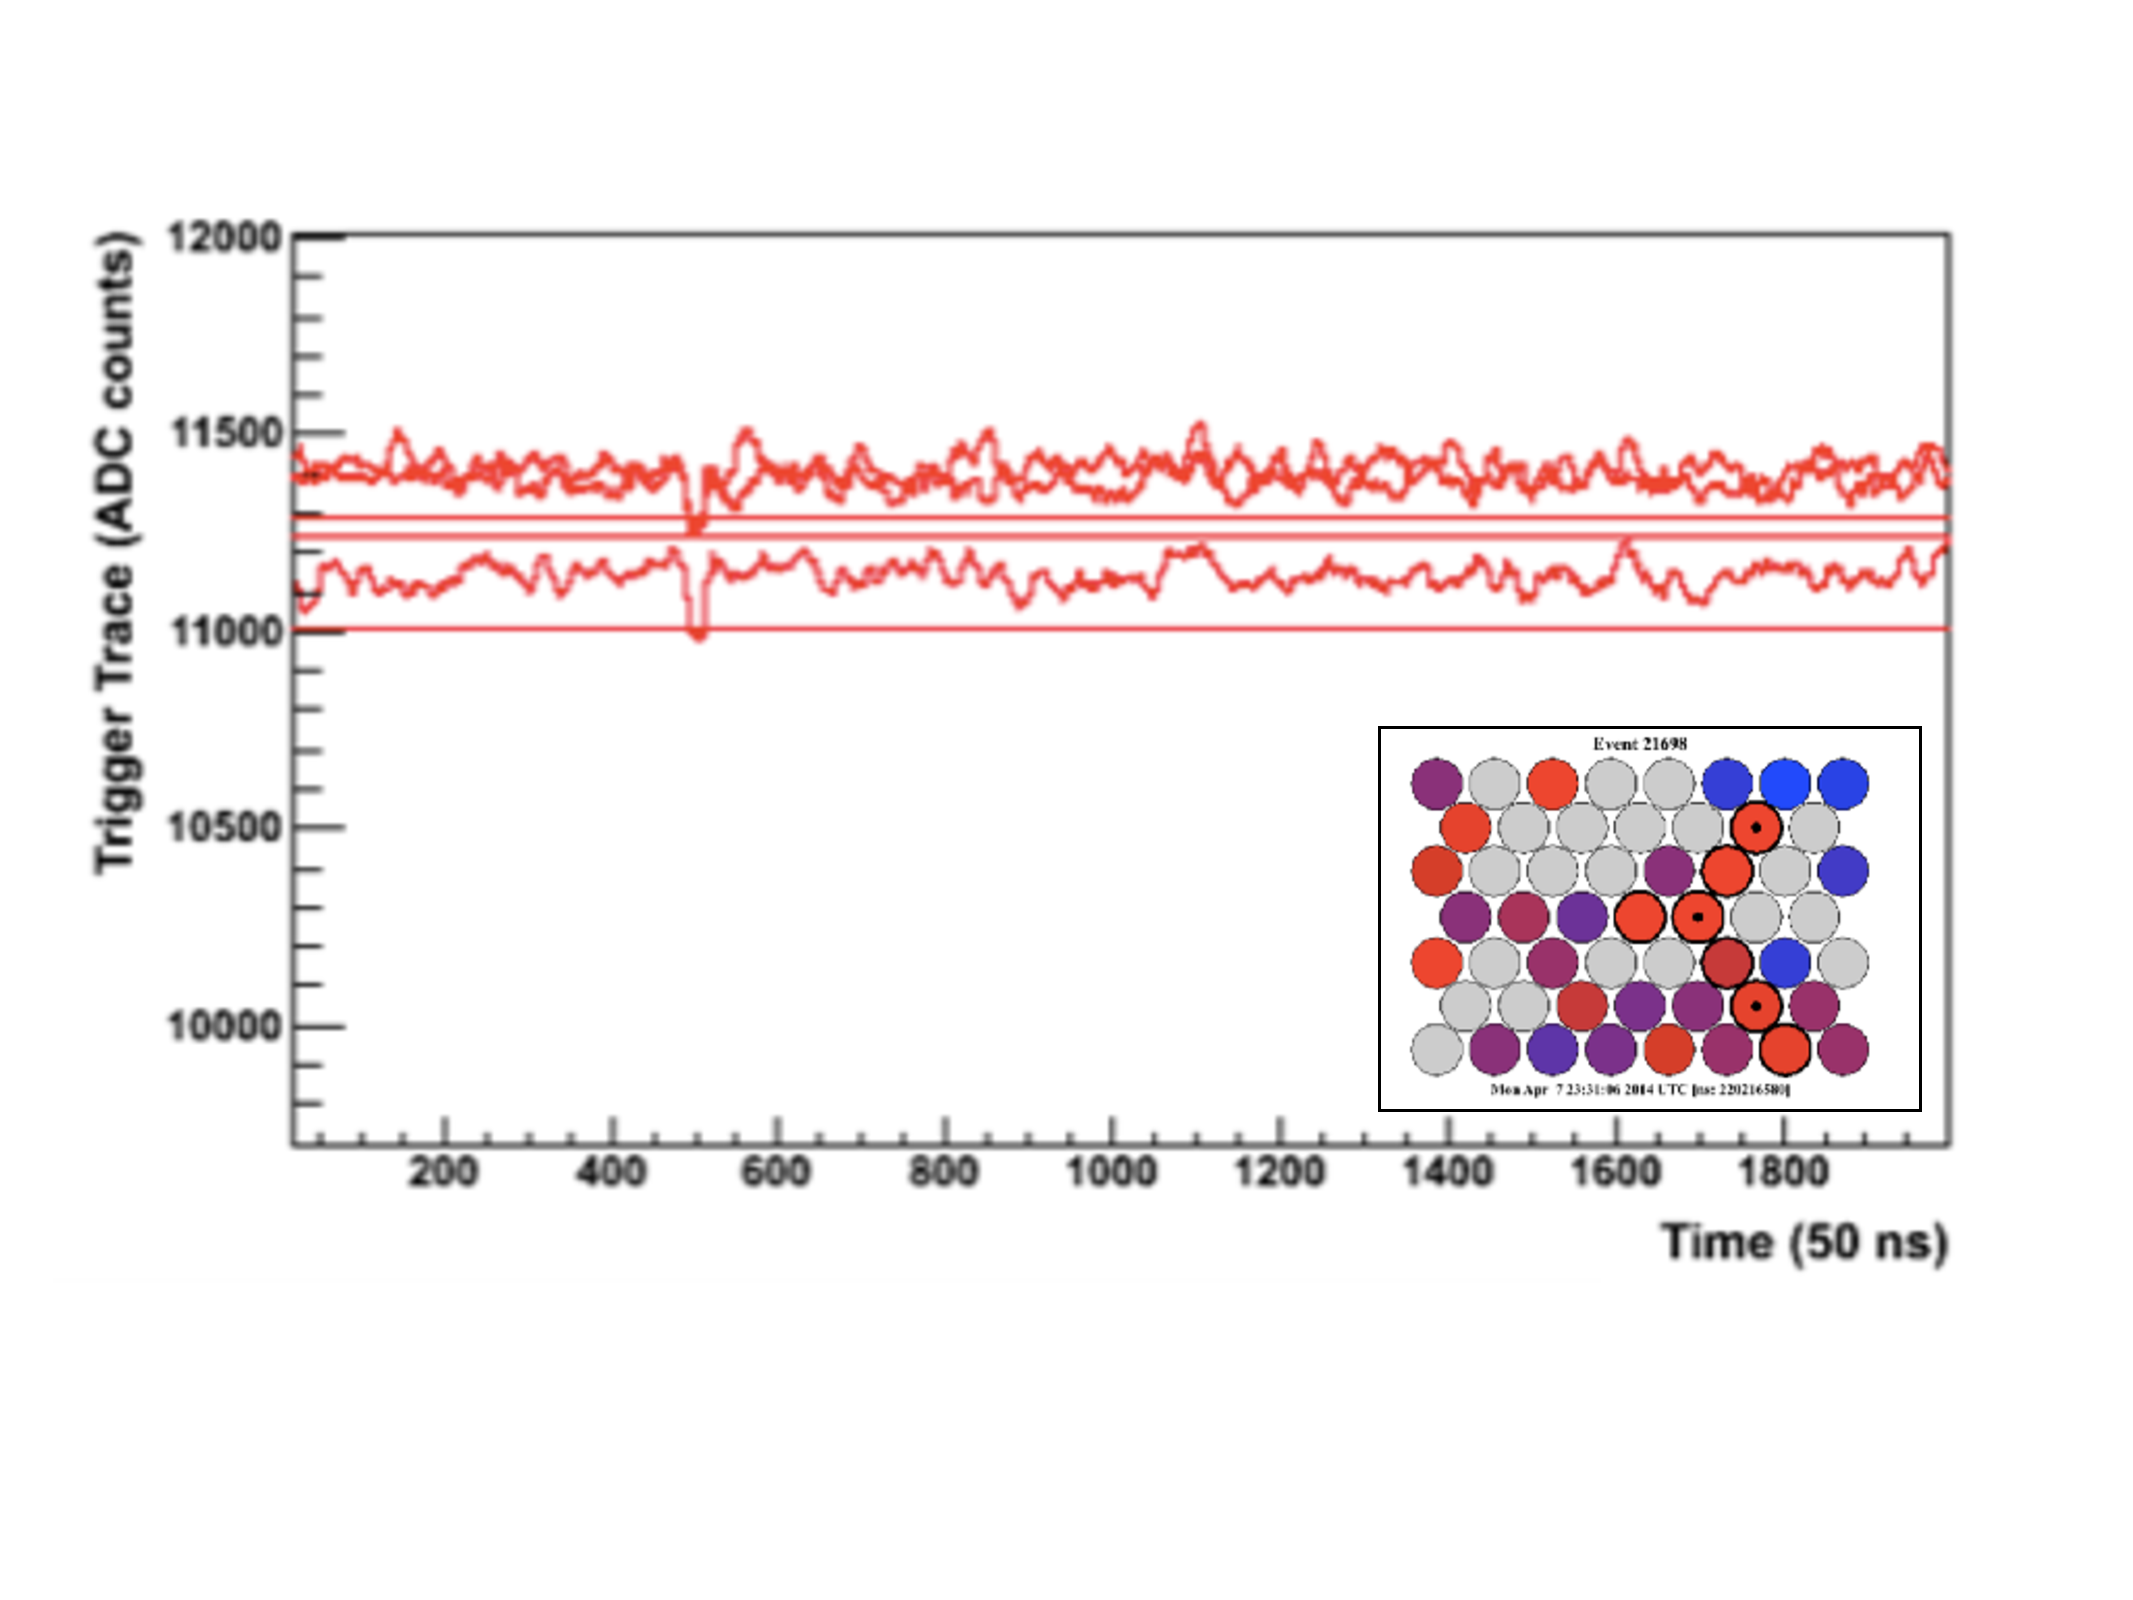
\includegraphics[width=0.49\textwidth]{midas_candidate_mix.pdf}
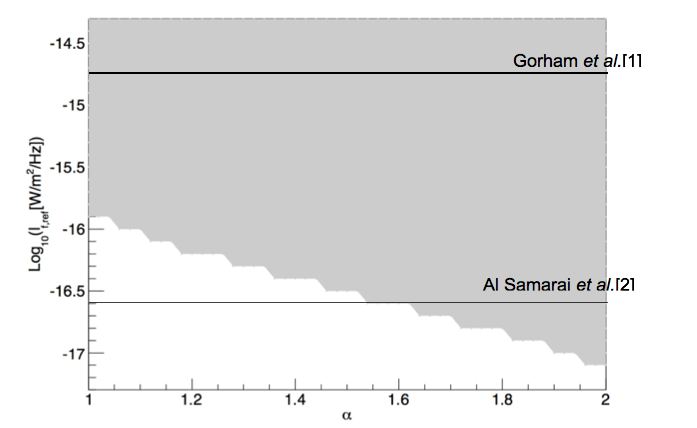
\includegraphics[width=0.49\textwidth]{midas_limit.png}
\caption{•}
\label{fig:midas_canditate}
\end{figure}

%The time difference of Auger and MIDAS events over 
%a large window of two seconds is shown in the 
%Figure~\ref{fig:midascoinc} and illustrate the 
%absence of an excess around zero. 
\section{Discussion and conclusions}
Two setups, EASIER and MIDAS, aiming at the observation of the  Molecular Bremstrahlung Radiation in coincidence with event detected at the Pierre Auger Observatory were presented. We presented a search for Ultra High Energy (E > 1EeV) EAS events in these setups. While clear radio events were observed in the radio surface detector EASIER, no signal were found with MIDAS microwave telescope. These results are however compatible if one considers other emissions origin. Indeed, the radio signal observed with EASIER are all from closeby showers and might be attributed to coherent emissions known to be dominant at lower frequencies. 



\begin{thebibliography}{99}
\bibitem{augerupgrade}Daniele Martello,The Pierre Auger Observatory Upgrade, CRI203, These Proc.
\bibitem{gorham}
First reference etc.

\end{thebibliography}

\end{document}
